\DiaryEntry{Queuing Theory, 1}{2019-08-04}{Stochastic}

This model is based on "Performance Modeling and Design of COmputer Systems", Chapter 8.10.

We are given an unbounded queue at which jobs arrive in discrete time steps. Suppose that with probability $p$ a job arrives, gets (maybe) queued, and, independently, with probability $q$ a job departs.

We model the queue as a discrete time markov chain, where the state is the (possibly inifnite) length of the qeue. The queue increases by one with probability $r = p(1-q)$ and decreases with probability $s = q(1-p)$. The markov chain looks as follows   


\begin{figure}[hbt!]
\centering
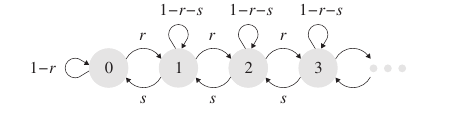
\includegraphics[scale=0.75]{images/queuing_01_01.png}
\end{figure}

The corresponding transition probability matrix is infinite (as the MC has inifnite states),

\bee
\Pbf = \begin{pmatrix}
1-r &    r & 0 & 0 & \cdots \\
s  & 1-r-s & r & 0 & \cdots \\
0  & s     & 1-r-s & r \\
0 & 0 & s & 1-r-s \\
\cdots & \cdots & \cdots & \cdots
\end{pmatrix}
\eee

We are interested in the stationary probabilities $\pi = [\pi_0 \pi_1 \cdots]$ which are given by

\bee
\pi P = \pi
\eee

and which yield the following (infinite) set of equations,

\begin{align*}
\pi_0 &= \pi_0 (1-r) + \pi_1 s \\ 
\pi_1 &= \pi_0 r + \pi_1(1-r-s) + \pi_2 s \\
\pi_2 &= \pi_1 r + \pi_2(1-r-s) + \pi_3 s \\
\pi_3 &= \pi_2 r + \pi_3(1-r-s) + \pi_4 s \\
\vdots
\end{align*} 

together with the "normalization", equation $\sum_i \pi_i = 1$. From the first equation we see that $\pi_1 = r/s \pi_0$, which we can insert into the second one etc. We finally arrive at

\bee
\pi_i = \left( \frac{r}{s} \right)^i \pi_0
\eee

To obtain an expression for $\pi_0$ e use the "normalization" equation,

\bee
\pi_0 \left(1 + \frac{r}{s} + \frac{r^2}{s^2} + \cdots \right) = 1
\eee

with the sum being solved by the geometric sum formula,

\bee
\pi_0 \frac{1}{1 - \frac{r}{s}} = 1 \rightarrow \pi_0 = 1 - \frac{r}{s}
\eee

and therefore

\bee
\pi_i = \left( \frac{r}{s} \right)^i \left( 1 - \frac{r}{s} \right) = \rho^i (1-\rho) \qed
\eee

where we have set $\rho = r/s$. We are next interested in the expected queue length,

\begin{align*}
E &= 1 \rho(1-\rho) + 2 \rho^2(1-\rho)+  3 \rho^3(1-\rho) + \cdots \\
  &= (1-\rho) \rho (1+2\rho + 3 \rho^2 + 4 \rho^3 + \cdots) \\
  &= (1-\rho) \rho \frac{d}{d\rho} (1 + \rho + \rho^2 + \rho^3 + \cdots) \\
  &= (1-\rho) \rho \frac{d}{d\rho} \frac{1}{1 - \rho} \\
  &= (1-\rho) \rho \frac{1}{(1-\rho)^2} = \frac{\rho}{1 - \rho} \qed
\end{align*}

Simulation can be found \href{https://github.com/ClemensFMN/JuliaStuff/blob/master/SimJulia/discrete_time_queue.jl}{here}. Basic idea is to realize that the state transitions are governed by a categorical distribution (which, howeve,r is different for the zero-state and all other states) with probabilities according to above Figure.


%%% Local Variables:
%%% mode: latex
%%% TeX-master: "journal"
%%% End:
